% Created 2017-12-14 jeu. 13:46
% Intended LaTeX compiler: pdflatex
\documentclass[10pt,svgnames,fragile]{beamer}
               \usepackage[frenchb]{babel}
\usepackage[utf8x]{inputenc}
\usepackage{lmodern}
\usepackage[T1]{fontenc}
\usepackage{graphicx}
\usepackage{etex}
\usepackage[usenames]{color}
\usepackage{xcolor}
\usepackage[normalem]{ulem}
\usepackage{textcomp}
\usepackage{pdflscape}
\usepackage{marvosym}
\usepackage{wasysym}
\usepackage{amssymb}
\usepackage{amsmath}
\usepackage{amsthm}
\usepackage{qtree}
\usepackage{bussproofs}
\usepackage{proof}
\usepackage{fitch}
\usepackage{cancel}
\usepackage{url}
\usepackage{smfthm}
\usepackage{multicol}
\useoutertheme{tree}

%% le code qui suit permet le rappel du plan à chaque changement de section:
\AtBeginSection[]{\begin{frame}<beamer>\frametitle{}\tableofcontents[currentsection,hideothersubsections]\end{frame}}
\subtitle{}

%%\titlegraphic{\includegraphics[height=1.5cm]{udl}}
\institute[Tecnológico de Costa Rica]{ Project 5: Linear Programming Problems \\ Second Semester 2018 }	       \usetheme{CambridgeUS}
\usepackage{beamer_udl_theme}
\setbeamertemplate{navigation symbols}{%
	%insertslidenavigationsymbol%
	%insertframenavigationsymbol%
	%insertsubsectionnavigationsymbol%
	%insertsectionnavigationsymbol%
	%insertdocnavigationsymbol%
	%insertbackfindforwardnavigationsymbol%
}
\usetheme{default}
\author{
Bryan Jiménez -\\ 
Patrick Maynard -\\ 
Dario Monestel -\\
} % Your name
\date{October 18}
\title[Operations research]{Operations research}
\begin{document}

\maketitle

\AtBeginSection{
\begin{frame}
  \frametitle{Index}
  \begin{multicols}{2}
  \tableofcontents[currentsection]
  \end{multicols}  
\end{frame}
}

\section{Problem 1}
\label{sec:org4f3d757}
\begin{frame}[label={sec:orge9abdcb}]{}
%%\begin{frame}

\frametitle{Problem 1}
Shale Oil, located on the island of Aruba, has a capacity of \textcolor{red}{600,000} barrels of crude oil per day. The final products from the refinery include two types of unleaded gasoline; regular and premium. The refining process encompasses four stages:

(1) The pure crude flows through a distillation tower that produces a feedstock.

(2) The feedstock output breaks up into two paths; the first path involves feedstock flowing into a cracker unit that refines the mixture into a gasoline stock. The second path has a portion of the feedstock flowing into the blender unit.

(3) The gasoline stock (from the cracker unit) feeds into the blender.

(4) The blender unit produces the final product, \textcolor{red}{regular or premium gasoline}.
\begin{figure}

\includegraphics[width=0.5\textwidth]{images/A.jpg}
\end{figure}

\end{frame}




\begin{frame}
\frametitle{Problem 1}
\framesubtitle{cont}
Both the regular and premium gasoline can be produced from either the feedstock or the gasoline stock during the blending process, although at different production costs. The company estimates that the net profit per barrel of regular gasoline is \textcolor{red}{6.20 \$} from feedstock and \textcolor{red}{8.80 \$} from gasoline stock. The corresponding profit values for the premium are \textcolor{red}{11.40 \$} from the feedstock and \textcolor{red}{10.30 \$} from the gasoline stock. According to design specifications, it takes five barrels of crude oil to produce one barrel of feedstock. The cracker units cannot use more than \textcolor{red}{30,000} barrels of feedstock per day. All remaining feedstock is used directly in the blender unit to produce the end product gasoline. The demand limits for regular and premium gasoline are \textcolor{red}{90,000} and \textcolor{red}{60,000 barrels per day}.



\end{frame}
%------------------------------------------------
 %------------------------------------------------
\begin{frame}[label={sec:orge9abdcb}]{}
%%\begin{frame}

\frametitle{Problem 1: decision variables}

X1: Regular gasoline from crude oil\\
X2: Premium gasoline from crude oil\\
X3: Regular gasoline coming from the disintegration\\
X4: Premium gasoline from the disintegration\\

\end{frame}

\begin{frame}[label={sec:orge9abdcb}]{}
%%\begin{frame}

\frametitle{Problem 1:  Objective Function }
\textcolor{red}{Maximize}\\[1em]
Z = 7.7X1 + 10.40X2 + 5.20X3 + 12.3X4\\

\end{frame}

\begin{frame}[label={sec:orge9abdcb}]{}
%%\begin{frame}

\frametitle{Problem 1:  Constraints }

X3 + X4 <= 40000\\
X1 + X3 <= 80000\\
X2 + X4 <= 50000\\
5X1 + 5X2 + 5X3 + 5X4 <= 600000\\
X1,X2,X3,X4 >= 0

\end{frame}

\begin{frame}[label={sec:orge9abdcb}]{}
%%\begin{frame}

\frametitle{Problem 1: Full Model }
\textcolor{red}{Maximize}\\[1em]

Z = 7.7X1 + 10.40X2 + 5.20X3 + 12.3X4\\[1em]


\textcolor{red}{subject to:}\\[1em]
X3 + X4 <= 40000\\
X1 + X3 <= 80000\\
X2 + X4 <= 50000\\
5X1 + 5X2 + 5X3 + 5X4 <= 600000\\
X1,X2,X3,X4 >= 0

\end{frame}

\begin{frame}[label={sec:orge9abdcb}]{}
%%\begin{frame}

\frametitle{Problem 1: Solution with Lingo }
%\textcolor{yellow}{Model problem}\\
\begin{figure}
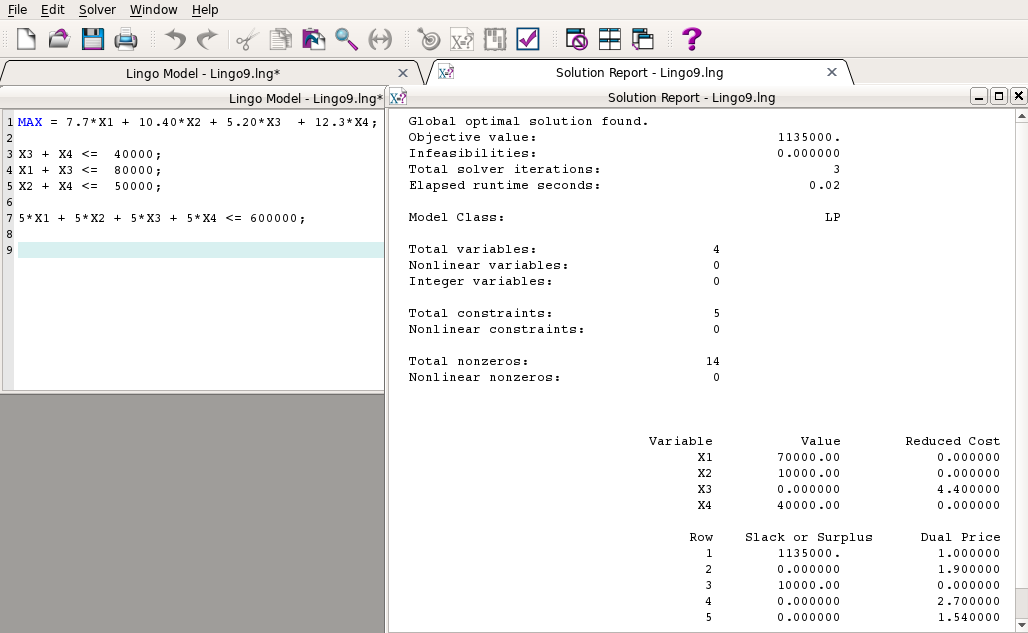
\includegraphics[width=0.7\textwidth]{images/1.png}
\end{figure}


\end{frame}


\begin{frame}[label={sec:org9c62e72}]{}
%%\begin{frame}
\frametitle{Problem 1: Final Solution}

X1 = 70000\\
X2 = 10000\\
X3 = 0\\
X4 = 40000\\
Z = 1135000
\end{frame}

\section{Problem 2}
\label{sec:org924d969}
\begin{frame}[label={sec:org9c62e72}]{}
%%\begin{frame}
\frametitle{Problem 2}


Hawaii Sugar Company produces brown sugar, processed sugar (white), powdered sugar and molasses with sugar cane syrup. The company buys \textcolor{red}{4000 tons} of syrup a week and has a contract to deliver a minimum of \textcolor{red}{25 tons} per week of each type of sugar. The production process starts with making brown sugar and molasses with the syrup. One ton of syrup produces \textcolor{red}{0.3 tons} of brown sugar and \textcolor{red}{0.1 tons} of molasses. Afterwards, the white sugar is made by processing brown sugar.

\begin{figure}
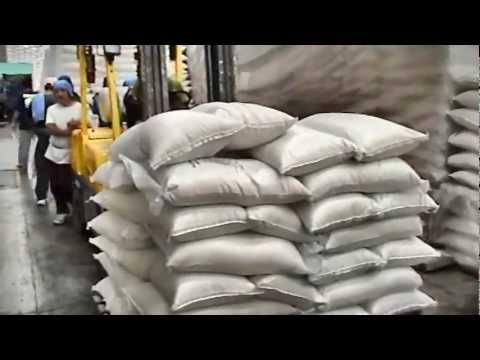
\includegraphics[width=0.5\textwidth]{images/B.jpg}
\end{figure}


\end{frame}


\begin{frame}[label={sec:org9c62e72}]{}
%%\begin{frame}
\frametitle{Problem 2}
\framesubtitle{cont}

It requires \textcolor{red}{0.1 tons} of brown sugar to produce \textcolor{red}{0.8 tons} of white sugar. Finally, powdered sugar is made from white sugar by means of a special milling process, which has \textcolor{red}{95 \%} conversion efficiency (1 ton of white sugar produces \textcolor{red}{.95 tons} of powdered sugar). The profits per ton of brown sugar, white sugar, powdered sugar and molasses are \textcolor{red}{150}, \textcolor{red}{200}, \textcolor{red}{230} and \textcolor{red}{35 \$}, respectively.



\end{frame}


%------------------------------------------------



\begin{frame}[label={sec:orge9abdcb}]{}
%%\begin{frame}

\frametitle{Problem 2: decision variables }

X1 = Tons brown sugar \\
X2 = Tons white sugar \\
X3 = Tons of powdered sugar \\
X4 = Tons molasses

\end{frame}

\begin{frame}[label={sec:orge9abdcb}]{}
%%\begin{frame}

\frametitle{Problem 2: Objective Function }
Maximize\\[1em]

Z =  150X1 + 200X2 + 230X3 + 35X4


\end{frame}

\begin{frame}[label={sec:orge9abdcb}]{}
%%\begin{frame}

\frametitle{Problem 2: Constrains }
	X1 >= 25\\
	X2 >= 25\\
	X3 >= 25\\
	X4 >= 25\\
	X4 <= 400\\
	
	0.76X1 + 0.95X2 + X3 <= 912


\end{frame}

\begin{frame}[label={sec:orge9abdcb}]{}
%%\begin{frame}

\frametitle{Problem 2: Full Model }
\textcolor{red}{Maximize}\\

Maximize\\[1em]

Z =  150X1 + 200X2 + 230X3 + 35X4


\textcolor{red}{subject to:}\\
	X1 >= 25\\
	X2 >= 25\\
	X3 >= 25\\
	X4 >= 25\\
	X4 <= 400\\
	
	0.76*X1 + 0.95*X2 + X3 <= 912

\end{frame}

\begin{frame}[label={sec:orge9abdcb}]{}
%%\begin{frame}

\frametitle{Problem 2: Solution with Lingo }
%\textcolor{yellow}{Model problem}\\
\begin{figure}
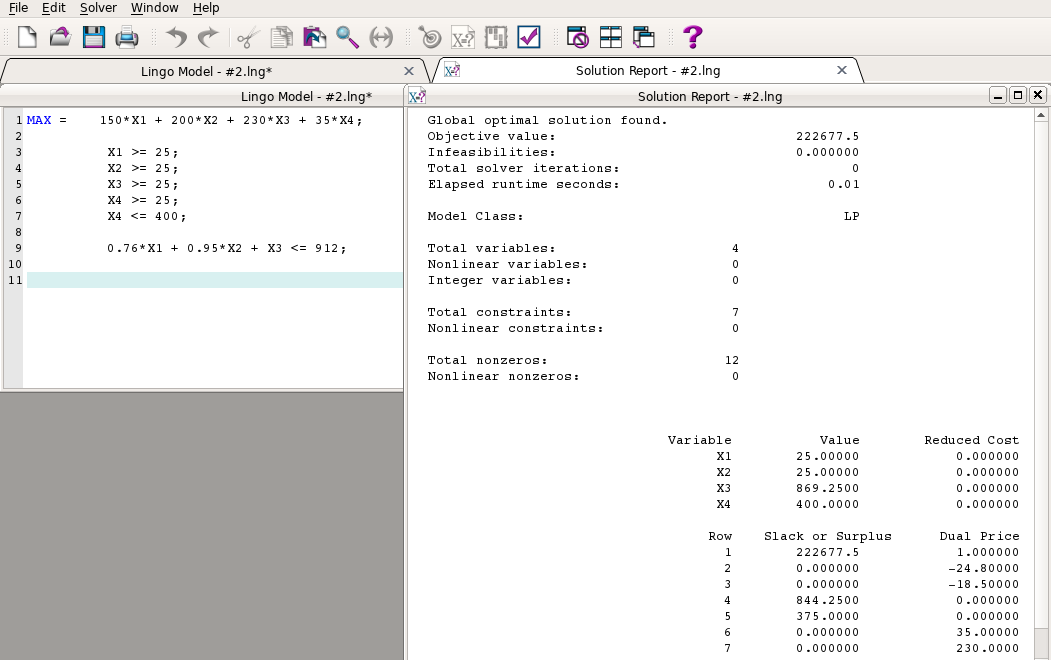
\includegraphics[width=0.7\textwidth]{images/2.png}
\end{figure}


\end{frame}

\begin{frame}[label={sec:org9c62e72}]{}
%%\begin{frame}
\frametitle{Problem 2: Final Solution}

X1 = 25\\
X2 = 25\\
X3 = 869\\
X4 = 400\\
Z = 222677.5
\end{frame}



%%%%%%

\section{Problem 3}
\label{sec:org92dd686}
%------------------------------------------------

\begin{frame}
\frametitle{Problem 3}

Fox Companies plans \textcolor{red}{six possible construction projects} during the following \textcolor{red}{4 years}. The following table shows the expected revenues (at present value) and the cash disbursements for those projects. Fox is authorized to undertake any of the projects, partially or totally. A partial termination of a project will have income and proportional disbursements.

\begin{figure}

\includegraphics[width=0.5\textwidth]{images/C.jpg}
\end{figure}



\end{frame}

%------------------------------------------------

\begin{frame}

\frametitle{Problem 3}
\framesubtitle{cont}
\begin{figure}
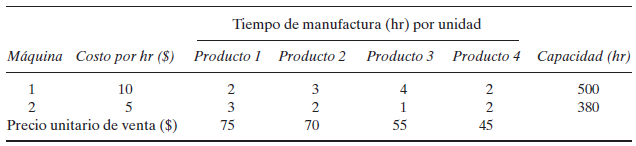
\includegraphics[width=0.7\textwidth]{images/io3.PNG}
\end{figure}
\end{frame}

%  Analysis problem 3

\begin{frame}[label={sec:orge9abdcb}]{}
\frametitle{Problem 3: decision variables }

x1: Amount of project 1 to undertake\\
x2: Amount of project 2 to undertake\\
x3: Amount of project 3 to undertake\\
x4: Amount of project 4 to undertake\\
x5: Amount of project 5 to undertake\\
x6: Amount of project 6 to undertake\\


\end{frame}


\begin{frame}[label={sec:orge9abdcb}]{}
%%\begin{frame}

\frametitle{Problem 3: Objective Function }
Maximize\\[1em]

Z =  32.40x1+35.80x2+17.75x3+14.80x4+18.20x5+12.35x6


\end{frame}

\begin{frame}[label={sec:orge9abdcb}]{}
\frametitle{Problem 3: Constrains }
\textcolor{red}{Funds available in year 1.}\\

10.5X1 + 8.3X2 + 10.2X3 + 7.2X4 + 12.3X5 + 9.2X6 <= 60\\

\textcolor{red}{Funds available in year 2.}\\

14.4X1 + 12.6X2 + 14.2X3 + 10.5X4 + 10.1X5 + 7.8X6 <= 70\\

\textcolor{red}{Funds available in year 3.}\\

2.2X1 + 9.5X2 + 5.6X3 + 7.5X4 + 8.3*X5 + 6.9X6 <= 35\\

\textcolor{red}{Funds available in year 4.}\\
2.4X1 + 3.1X2 + 4.2X3 + 5X4 + 6.3X5 + 5.1X6 <= 20


\textcolor{red}{positive values}\\
x1, x2, x3, x4, x5, x6 >= 0




\end{frame}

\begin{frame}[label={sec:orge9abdcb}]{}
\frametitle{Problem 3: Full Model }
\textcolor{red}{Maximize}\\[1em]
Z = 32.40X1 + 35.80X2 + 17.75X3 + 14.80X4 + 18.20X5 + 12.35X6\\[1em]
\textcolor{red}{subject to:}\\[1em]

10.5X1 + 8.3X2 + 10.2X3 + 7.2X4 + 12.3X5 + 9.2X6 <= 60\\
14.4X1 + 12.6X2 + 14.2X3 + 10.5X4 + 10.1X5 + 7.8X6 <= 70\\
2.2X1 + 9.5X2 + 5.6X3 + 7.5X4 + 8.3*X5 + 6.9X6 <= 35\\
2.4X1 + 3.1X2 + 4.2X3 + 5X4 + 6.3X5 + 5.1X6 <= 20
\end{frame}

\begin{frame}[label={sec:orge9abdcb}]{}
%%\begin{frame}
\frametitle{Problem 3 Solution with Lingo }
%\textcolor{yellow}{Model problem}\\
\begin{figure}
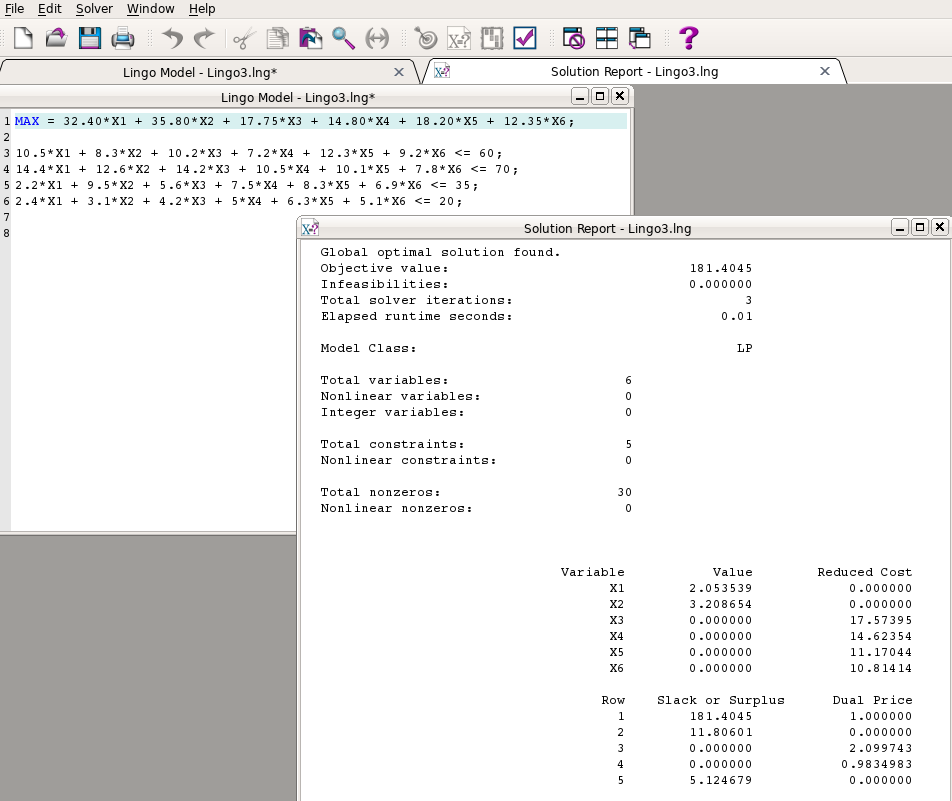
\includegraphics[width=0.7\textwidth]{images/3.png}
\end{figure}
\end{frame}

\begin{frame}[label={sec:org9c62e72}]{}
%%\begin{frame}
\frametitle{Problem 3: Final Solution}

X1 = 2.05\\
X2 = 3.20\\
X3 = 0\\
X4 = 0\\
X5 = 0\\
X6 = 0\\
Z = 181.40 
\end{frame}


\section{Problem 4}
\label{sec:org92dd686}



\begin{frame}
\frametitle{Problem 4}

Manufacturing Acme received a contract to deliver housing windows for the following \textcolor{red}{6 months}. The successive demands for the \textcolor{red}{six periods} are \textcolor{red}{100}, \textcolor{red}{250}, \textcolor{red}{190}, \textcolor{red}{140}, \textcolor{red}{220} and \textcolor{red}{110}, respectively. The cost of production per window varies from month to month, depending on the costs of labor, materials and services. Acme estimates that the production cost per window, during the following 6 months, will be  \textcolor{red}{50}, \textcolor{red}{45}, \textcolor{red}{55}, \textcolor{red}{48}, \textcolor{red}{52} and \textcolor{red}{50} dollars, respectively. To take advantage of fluctuations in the cost of manufacturing, Acme could choose to produce more than necessary in a given month, and save surplus units to deliver in later months. However, this will result in a storage cost of \textcolor{red}{8 \$ per window and per month}, evaluated with the inventory raised at the end of the month.

\begin{figure}
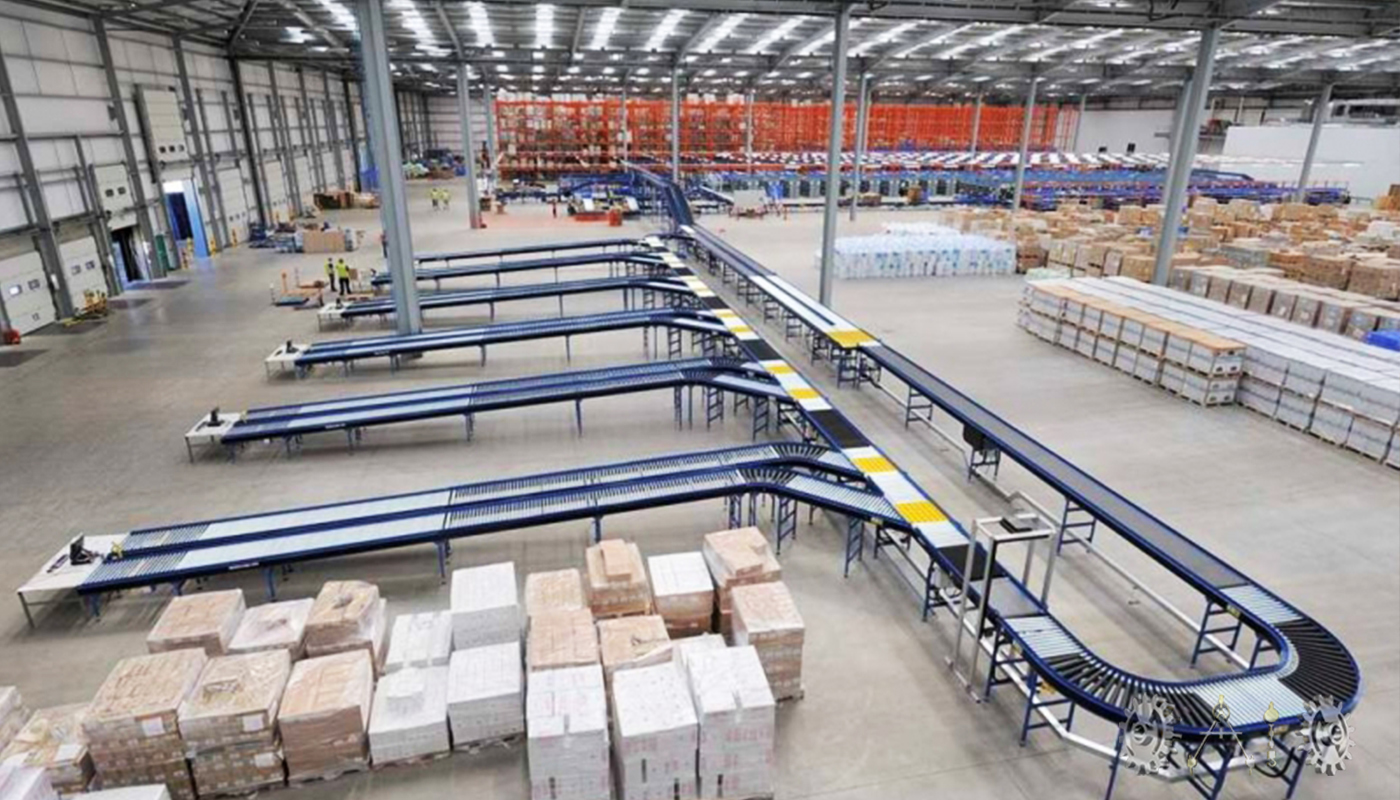
\includegraphics[width=0.4\textwidth]{images/D.jpg}
\end{figure}

\end{frame}

% Analysis problem 4

\begin{frame}[label={sec:orge9abdcb}]{}
\frametitle{Problem 4: decision variables }

i = month number in this case 1,2,3,4,5,6 for 6 months\\

Xi = Number of units produced in month i\\

Ii = Units left in the end of month inventory i

\end{frame}

\begin{frame}[label={sec:orge9abdcb}]{}
%%\begin{frame}

\frametitle{Problem 4: Objective Function }
Minimize\\[1em]

Z = 50X1 + 45X2 + 55X3 + 48X4 + 52X5 + 50X6 +\\ 8(W1 + W2 + W3 + W4 + W5 + W6)\\


\end{frame}

\begin{frame}[label={sec:orge9abdcb}]{}
\frametitle{Problem 4: Constrains }

x1 - W1 = 100\\ 

W1 + X2 - W2 = 250\\

W2 + X3  - W3 = 190\\

W3 + X4 - W4 = 140·\\

W4 + X5 - W5 = 220\\

I5 + X6 = 110\\




\end{frame}

\begin{frame}[label={sec:orge9abdcb}]{}
\frametitle{Problem 4: Full Model }
\textcolor{red}{Minimize}\\[1em]

Z = 50X1 + 45X2 + 55X3 + 48X4 + 52X5 + 50X6 +\\ 8(W1 + W2 + W3 + W4 + W5 + W6)\\[1em]
\textcolor{red}{subject to:}\\[1em]
x1 - W1 = 100\\ 

W1 + X2 - W2 = 250\\

W2 + X3  - W3 = 190\\

W3 + X4 - W4 = 140·\\

W4 + X5 - W5 = 220\\

I5 + X6 = 110\\

\end{frame}

\begin{frame}[label={sec:orge9abdcb}]{}
%%\begin{frame}

\frametitle{Problem 4: Solution with Lingo }
%\textcolor{yellow}{Model problem}\\
\begin{figure}
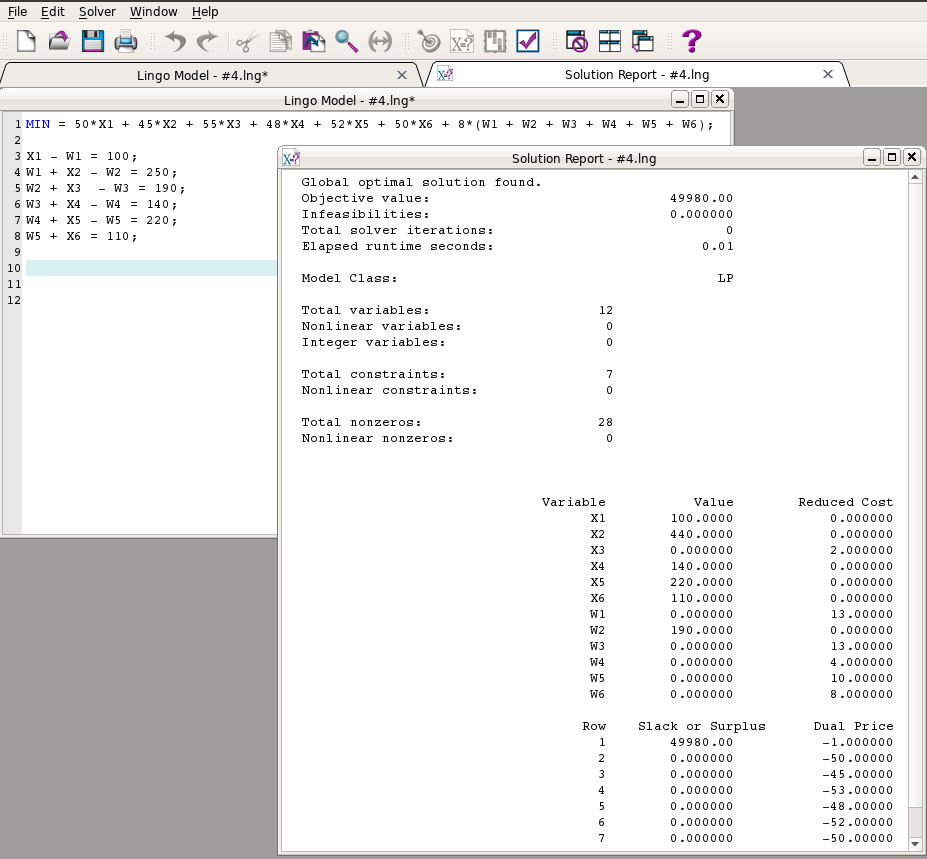
\includegraphics[width=0.7\textwidth]{images/4.png}
\end{figure}
\end{frame}


\begin{frame}[label={sec:org9c62e72}]{}
%%\begin{frame}
\frametitle{Problem 4: Final Solution}

X1 = 100\\
X2 = 440\\
X3 = 0\\
X4 = 140\\
X5 = 220\\
X6 = 110\\
W1 = 100\\
W2 = 440\\
W3 = 0\\
W4 = 140\\
W5 = 220\\
W6 = 110\\
Z = 49980
\end{frame}


\section{Problem 5}
\label{sec:org92dd686}


\begin{frame}
\frametitle{Problem 5}

Investor Doe has four potential opportunities to invest a total of \textcolor{red}{100,000 \$}. The following table provides the cash flow for four investments.

\begin{figure}
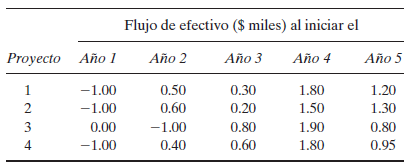
\includegraphics[width=0.7\textwidth]{images/io1.PNG}
\end{figure}
\end{frame}

\begin{frame}
\frametitle{Problem 5}
\framesubtitle{cont}

The information in this table can be interpreted as follows:

for project 1, \textcolor{red}{1.00 \$} invested at the beginning of year 1, it will yield \textcolor{red}{0.50 \$} at the beginning of year 2, \textcolor{red}{0.30 \$} at the beginning of year 3, \textcolor{red}{1.80 \$} at the beginning of year 4 and \textcolor{red}{1.20 \$} at the beginning of year 5. The remaining elements can be interpreted in analogous
A case without transactions is indicated by a 0.00 element. Juan also has the option of investing in a bank account that produces \textcolor{red}{6.5\%} per year. The funds accumulated in a year can be reinvested in the following years.

\begin{figure}

\includegraphics[width=0.4\textwidth]{images/E.jpg}
\end{figure}

\end{frame}

% Analysis problem 5

\begin{frame}[label={sec:orge9abdcb}]{}
\frametitle{Problem 5: decision variables }

Xi =  Dollars invested in the project 
i, i = 1,2,3,4

Yj = Dollars invested in the bank per year
j, j= 1,2,3,4,5



\end{frame}

\begin{frame}[label={sec:orge9abdcb}]{}
%%\begin{frame}

\frametitle{Problem 5: Objective Function }
Maximize\\[1em]

Z =  Y5


\end{frame}

\begin{frame}[label={sec:orge9abdcb}]{}
\frametitle{Problem 5: Constrains }
X1 + X2 + X4 + Y1 <= 100 000\\
0.5X1 + 0.6X2 - X3 + 0.4X4 + 1.065Y1 - Y2 = 0\\
0.3X1 + 0.2X2 - 0.8X3 + 0.6X4 + 1.065Y2 - Y3 = 0\\
1.8X1 + 1.5X2 - 1.9X3 + 1.8X4 + 1.065Y3 - Y4 = 0\\
1.2X1 + 1.3X2 - 0.8X3 + 0.95X4 + 1.065Y4 - Y5 = 0\\

Xi >= 0

\end{frame}

\begin{frame}[label={sec:orge9abdcb}]{}
\frametitle{Problem 5: Full Model }
\textcolor{red}{Maximize}\\[1em]

Z =  Y5\\[1em]
\textcolor{red}{subject to:}\\[1em]
X1 + X2 + X4 + Y1 <= 100 000\\
0.5X1 + 0.6X2 - X3 + 0.4X4 + 1.065Y1 - Y2 = 0\\
0.3X1 + 0.2X2 - 0.8X3 + 0.6X4 + 1.065Y2 - Y3 = 0\\
1.8X1 + 1.5X2 - 1.9X3 + 1.8X4 + 1.065Y3 - Y4 = 0\\
1.2X1 + 1.3X2 - 0.8X3 + 0.95X4 + 1.065Y4 - Y5 = 0\\
Xi >= 0
\end{frame}

\begin{frame}[label={sec:orge9abdcb}]{}
%%\begin{frame}
\frametitle{Problem 5 Solution with Lingo }
%\textcolor{yellow}{Model problem}\\
\begin{figure}
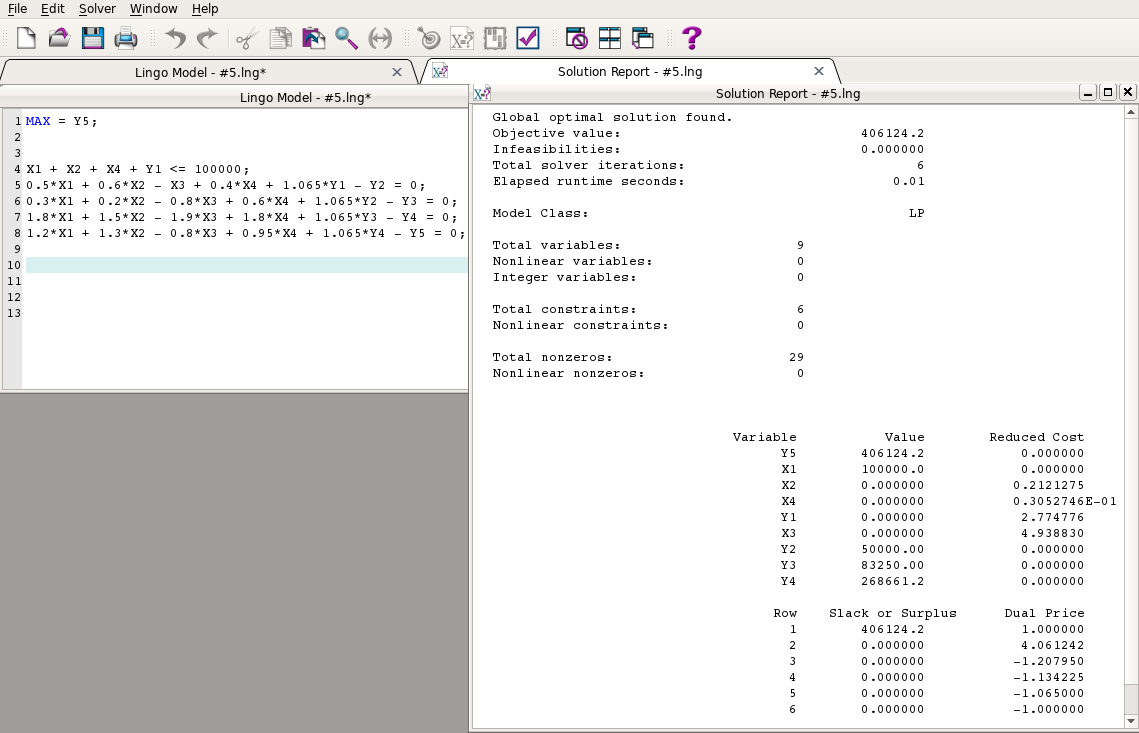
\includegraphics[width=0.7\textwidth]{images/5.png}
\end{figure}
\end{frame}

\begin{frame}[label={sec:org9c62e72}]{}
%%\begin{frame}
\frametitle{Problem 5: Final Solution}

X1 = 100000\\
X2 = 0\\
X3 = 0\\
X4 = 0\\
Y1 = 0\\
Y2 = 50000\\
Y3 = 83250\\
Y4 = 268661.2\\
Z = 406124
\end{frame}



\section{Problem 6}
\label{sec:org92dd686}


\begin{frame}
\frametitle{Problem 6}


Toolco has signed a contract with AutoMate to provide their discount automotive stores with chisels and wrenches. The weekly demand of AutoMate is \textcolor{red}{1500 wrenches} and \textcolor{red}{1200} chisels. Toolco's current capacity is not large enough to produce units the required units and must work overtime and possibly outsource to other tool shops.

The result is an increase in the cost of production per unit, as shown in the following table. The market restricts the wrenches to a ratio of at least 2: 1 with the chisels.

\begin{figure}

\includegraphics[width=0.3\textwidth]{images/F.png}
\end{figure}



\end{frame}

%------------------------------------------------

\begin{frame}
\frametitle{Problem 6}
\framesubtitle{cont}

\begin{figure}
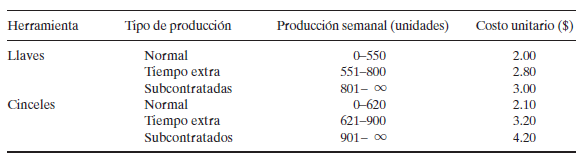
\includegraphics[width=0.7\textwidth]{images/io9.PNG}
\end{figure}


\end{frame}

% Analysis problem 6

\begin{frame}[label={sec:orge9abdcb}]{}
\frametitle{Problem 6: decision variables }

Kn: Number of keys produced in normal time\\
Ke: Quantity of keys produced in extra time\\
Ks: Number of keys by subcontract\\

Cn: Amount of Chisels produced in normal time\\
Ce: Quantity of Chisels produced in extra time\\
Cs: Quantity of Chisels by subcontract\\

\end{frame}

\begin{frame}[label={sec:orge9abdcb}]{}
%%\begin{frame}

\frametitle{Problem 6: Objective Function }
Minimize\\[1em]

Z = 2Kn + 2.8Ke + 3Ks + 2.1Cn + 3.2Ce + 4.2Cs



\end{frame}

\begin{frame}[label={sec:orge9abdcb}]{}
\frametitle{Problem 6: Constrains }

%2Xw1 + 2XW2 + 2XW3 - Xc1 - XC2 - Xc3 <= 0\\
-2Kn-2Ke-2Ks+Cn+Ce+Cs >= 0
Kn + Ke + Ks >= 1500\\
Cn + Ce + Cs >= 1200\\
Kn <= 550\\
Cn <= 620\\
Kn + Ke <= 800\\
Cn + Ce <= 900

\end{frame}

\begin{frame}[label={sec:orge9abdcb}]{}
\frametitle{Problem 6: Full Model }
\textcolor{red}{Minimize}\\[1em]


Z = 2Kn + 2.8Ke + 3Ks + 2.1Cn + 3.2Ce + 4.2Cs\\[1em]
\textcolor{red}{subject to:}\\[1em]
-2Kn-2Ke-2Ks+Cn+Ce+Cs >= 0
Kn + Ke + Ks >= 1500\\
Cn + Ce + Cs >= 1200\\
Kn <= 550\\
Cn <= 620\\
Kn + Ke <= 800\\
Cn + Ce <= 900

\end{frame}


\begin{frame}[label={sec:orge9abdcb}]{}

\frametitle{Problem 6: Solution with Lingo }
%\textcolor{yellow}{Model problem}\\
\begin{figure}
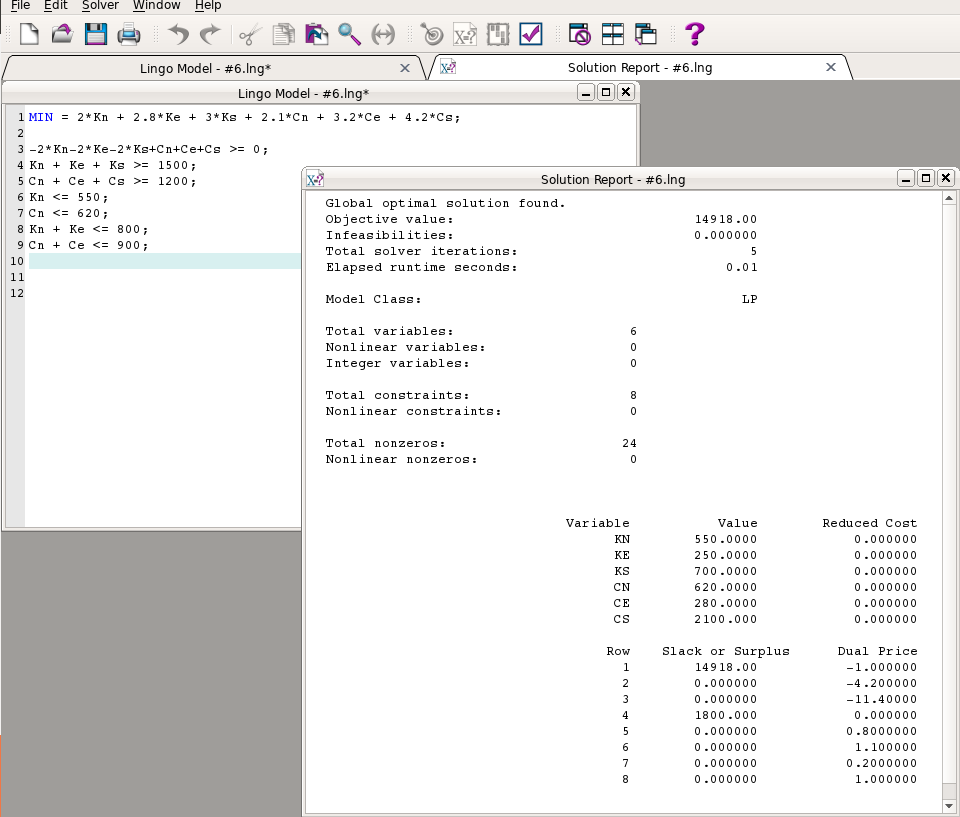
\includegraphics[width=0.7\textwidth]{images/6.png}
\end{figure}


\end{frame}

\begin{frame}[label={sec:org9c62e72}]{}
%%\begin{frame}
\frametitle{Problem 6: Final Solution}

Kn = 550\\
Ke = 250\\
Ks = 700\\
Cn = 620\\
Ce = 280\\
Cs = 2100\\
Z = 14918
\end{frame}


%------------------------------------------------
\section{Problem 7}
\label{sec:org92dd686}


\begin{frame}
\frametitle{Problem 7}


In \textcolor{red}{two machines}, four products are processed sequentially. The following table shows the relevant data of the problem.
\begin{figure}
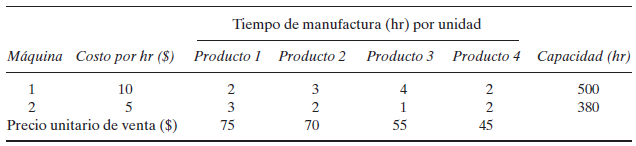
\includegraphics[width=0.7\textwidth]{images/io3.PNG}
\end{figure}\\




\end{frame}

% Analysis problem 7

\begin{frame}[label={sec:orge9abdcb}]{}
\frametitle{Problem 7: decision variables }\\[2em]

P1 : Product 1 \\
P2 : Product 2 \\
P3 : Product 3 \\
P4 : Product 4 \\[1em]

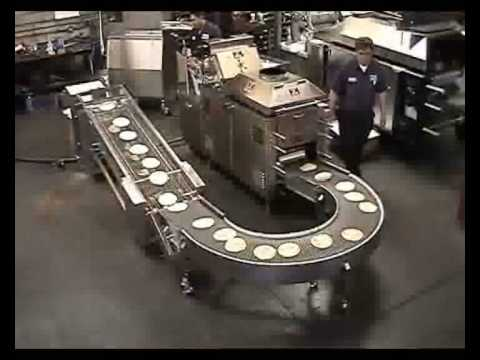
\includegraphics[width=0.4\textwidth]{images/G.jpg}
\end{figure}

\end{frame}

\begin{frame}[label={sec:orge9abdcb}]{}
%%\begin{frame}

\frametitle{Problem 7: Objective Function }
Maximize\\[1em]

Z = 30P1 + 30P2 + 20P3 +15P4



\end{frame}

\begin{frame}[label={sec:orge9abdcb}]{}
\frametitle{Problem 7: Constrains }


2P1 + 3P2 + 4P3 + 2P4 <= 500\\[1em]
3P1+ 2P2 + P3 + 2P4 <= 380


\end{frame}

\begin{frame}[label={sec:orge9abdcb}]{}
\frametitle{Problem 7: Full Model }
\textcolor{red}{Maximize}\\[1em]
Z = 30P1 + 30P2 + 20P3 +15P4\\[1em]
\textcolor{red}{subject to:}\\[1em]
2P1 + 3P2 + 4P3 + 2P4 <= 500\\
3P1+ 2P2 + P3 + 2P4 <= 380
\end{frame}


\begin{frame}[label={sec:orge9abdcb}]{}

\frametitle{Problem 7: Solution with Lingo }
%\textcolor{yellow}{Model problem}\\
\begin{figure}
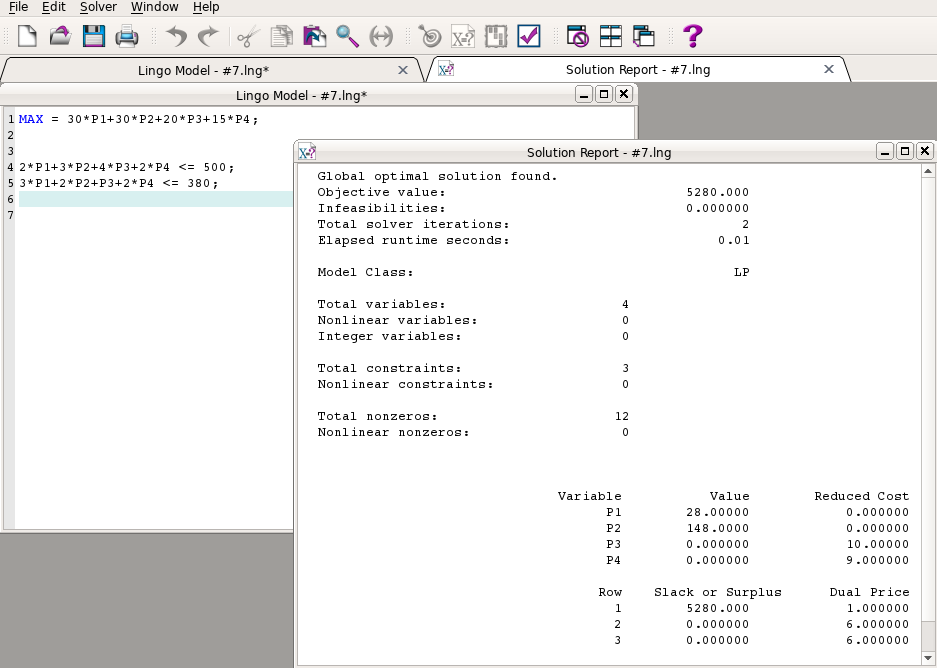
\includegraphics[width=0.7\textwidth]{images/7.png}
\end{figure}


\end{frame}

\begin{frame}[label={sec:org9c62e72}]{}
%%\begin{frame}
\frametitle{Problem 7: Final Solution}

P1 = 28\\
P2 = 148\\
P3 = 0\\
P4 = 0\\
Z = 5280
\end{frame}


%------------------------------------------------


\section{Problem 8}
\label{sec:org92dd686}

\begin{frame}
\frametitle{Problem 8}


A manufacturer produces \textcolor{red}{three models, I, II and III}, of a certain product, using the raw materials A and B. The following table shows the data for the problem.
\begin{figure}
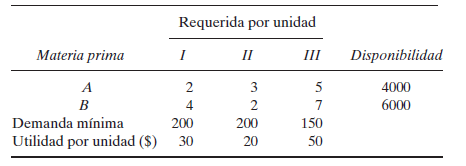
\includegraphics[width=0.7\textwidth]{images/io4.PNG}
\end{figure}


\end{frame}
%------------------------------------------------
\begin{frame}
\frametitle{Problem 8}
\framesubtitle{cont}\\[2em]

The labor time for model I is double that for II and triple of III. All factory personnel can produce the equivalent of \textcolor{red}{1500 model I units}. Market needs specify the 3: 2: 5 relationships of the productions of the three respective models.\\[2em]
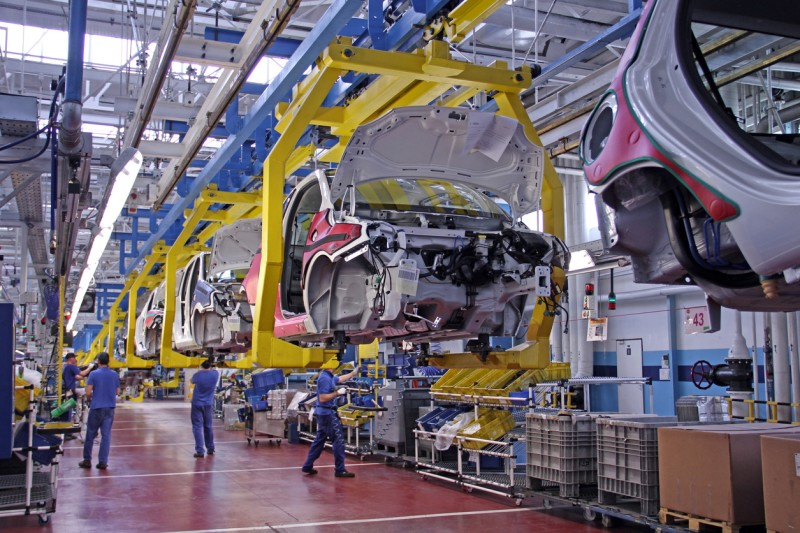
\includegraphics[width=0.5\textwidth]{images/H.jpeg}
\end{figure}

\end{frame}

% Analysis problem 8

\begin{frame}[label={sec:orge9abdcb}]{}
\frametitle{Problem 8: decision variables }

X1 = Units to be produced from the model product l\\

X2 = Units to be produced of the product model ll\\

X3 = Units to be produced of the model product lll

\end{frame}

\begin{frame}[label={sec:orge9abdcb}]{}
%%\begin{frame}

\frametitle{Problem 8: Objective Function }
Maximize\\[1em]

Z =  30X1 + 20X2 + 50X3


\end{frame}

\begin{frame}[label={sec:orge9abdcb}]{}
\frametitle{Problem 8: Constrains }
\textcolor{red}{Restriction of raw material A:} 2X1 + 3X2 + 5X3 <= 4000\\[1em]

\textcolor{red}{Restriction of raw material B :} 4X1 + 2X2 + 7X3 <= 6000\\[1em]

\textcolor{red}{Time restriction :} X1 + 0.5X2 + 0.33333 X3 <= 1500\\[1em]

\textcolor{red}{Production ratio in models l and ll:} 2X1 - 3X2 = 0\\[1em]

\textcolor{red}{Production ratio in models ll and lll:} 5X2 - 2X3 = 0\\[1em]

\textcolor{red}{Restriction of demand of the model l, ll, lll:}\\[1em]
X1,X2,x3  >= 200\\


X1,X2,X3   >= 0\\

\end{frame}

\begin{frame}[label={sec:orge9abdcb}]{}
\frametitle{Problem 8: Full Model }
\textcolor{red}{Maximize}\\[1em]

Z =  30X1 + 20X2 + 50X3[1em]

\textcolor{red}{subject to:}\\[1em]
2X1 + 3X2 + 5X3 <= 4000\\
4X1 + 2X2 + 7X3 <= 6000\\
X1 + 0.5X2 + 0.33333 X3 <= 1500\\
2X1 - 3X2 = 0
5X2 - 2X3 = 0
X1,X2,x3  >= 200\\
X1,X2,X3   >= 0\\

\end{frame}


\begin{frame}[label={sec:orge9abdcb}]{}

\frametitle{Problem 8: Solution with Lingo }
%\textcolor{yellow}{Model problem}\\
\begin{figure}
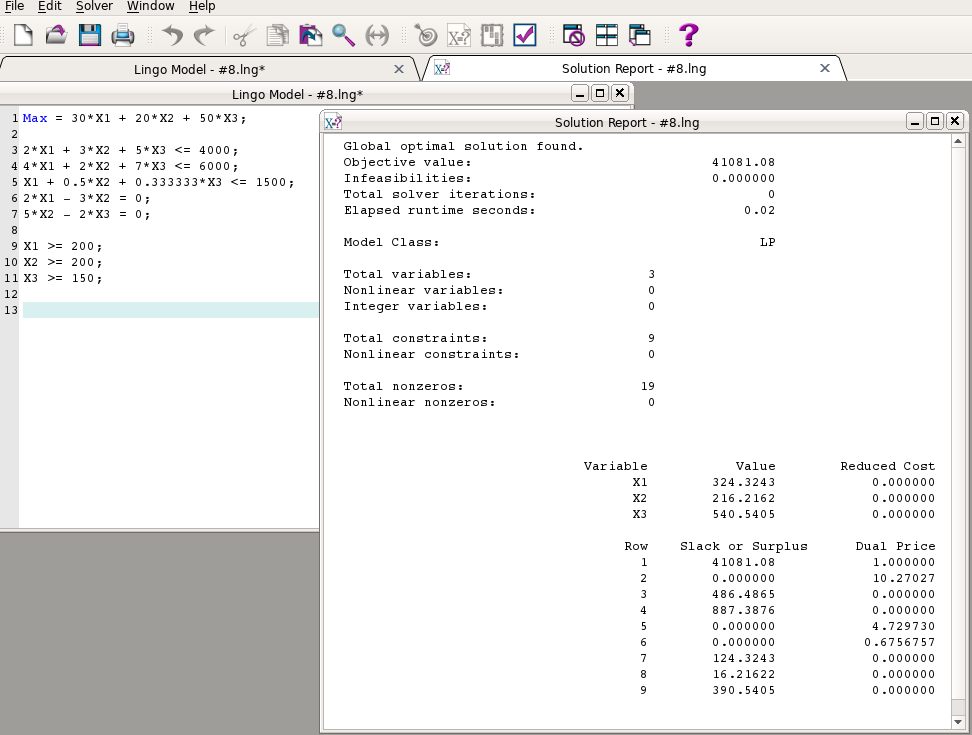
\includegraphics[width=0.7\textwidth]{images/8.png}
\end{figure}


\end{frame}


\begin{frame}[label={sec:org9c62e72}]{}
%%\begin{frame}
\frametitle{Problem 8: Final Solution}

X1 = 324\\
X2 = 216\\
X3 = 540\\
Z = 41081.08
\end{frame}

%------------------------------------------------

\section{Problem 9}
\label{sec:org92dd686}

\begin{frame}
\frametitle{Problem 9}


HiRise Construction can bid on two one-year projects. The quarterly cash flow (in millions of dollars) is provided in the following table for the \textcolor{red}{two projects}.
\begin{figure}
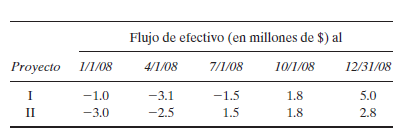
\includegraphics[width=0.7\textwidth]{images/io7.PNG}
\end{figure}
\end{frame}

%------------------------------------------------

\begin{frame}[fragile] % Need to use the fragile option when verbatim is used in the slide
\frametitle{Problem 9 }
\framesubtitle{cont}

HiRise has cash funds of \textcolor{red}{1 million} at the beginning of each quarter and can borrow an amount equal to \textcolor{red}{10\%} of the annual nominal interest rate. This means that if the \textcolor{red}{amount borrowed in quarter i is Bi then}. \[0 \leq B_{i} \leq 1, i = 1,2,3,4.\] 
Any borrowed money must be paid at the end of the quarter. The excess cash can earn a quarterly interest at a nominal annual rate of \textcolor{red}{8\%}. All the money accumulated at the end of a quarter is invested in the following quarter.\\[1em]

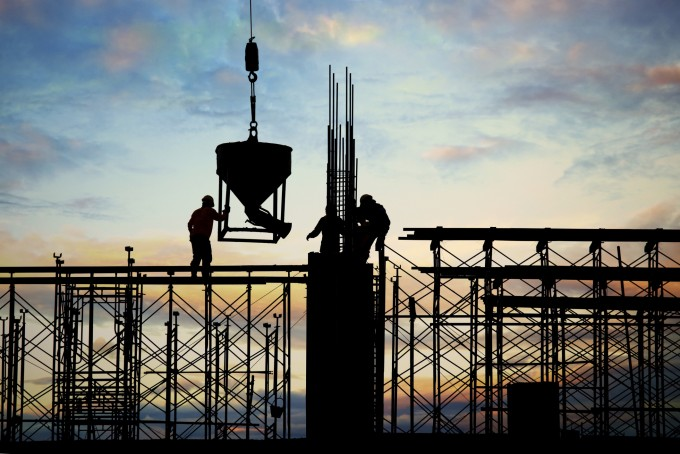
\includegraphics[width=0.5\textwidth]{images/I.jpg}
\end{figure}

\end{frame}

% Analysis problem 9

\begin{frame}[label={sec:orge9abdcb}]{}
\frametitle{Problem 9: decision variables }
Pi = Fraction undertaken from project i, 1 = 1,2\\
Bj = Millions of dollars loaned in semester j, j = 1,2,3,4\\
Sj = Surplus million dollars at the beginning of semester j, j = 1,2,3,4,5

\end{frame}

\begin{frame}[label={sec:orge9abdcb}]{}


\frametitle{Problem 9: Objective Function }
Maximize\\[1em]

Z = S5


\end{frame}

\begin{frame}[label={sec:orge9abdcb}]{}
\frametitle{Problem 9: Constrains }
P1 + 3P2 + S1 - B1 = 1\\
3.1P1 + 2.5P2 - 1.0S1 + S2 + 1.025B1 - B2 = 1\\
1.5P1 - 1.5P2 - 1.02S2 + S3 + 1.025B2 - B3 = 1\\
-1.8P1 - 1.8P2 - 1.02S3 + S4 + 1.025B3 - B4 = 1\\
-5P1 - 2.8P2 - 1.02S4 + S5 + 1.025B4 = 1\\

0 <= P1 <= 1\\
0 <= P2 <= 1\\
0 <= Bj <= 1  ,  j = 1,2,3,4

\end{frame}

\begin{frame}[label={sec:orge9abdcb}]{}
\frametitle{Problem 9: Full Model }
\textcolor{red}{Maximize}\\[1em]
Z = S5\\[1em]
\textcolor{red}{subject to:}\\[1em]
P1 + 3P2 + S1 - B1 = 1\\
3.1P1 + 2.5P2 - 1.0S1 + S2 + 1.025B1 - B2 = 1\\
1.5P1 - 1.5P2 - 1.02S2 + S3 + 1.025B2 - B3 = 1\\
-1.8P1 - 1.8P2 - 1.02S3 + S4 + 1.025B3 - B4 = 1\\
-5P1 - 2.8P2 - 1.02S4 + S5 + 1.025B4 = 1\\

0 <= P1 <= 1\\
0 <= P2 <= 1\\
0 <= Bj <= 1  ,  j = 1,2,3,4
\end{frame}


%------------------------------------------------
\begin{frame}[label={sec:orge9abdcb}]{}

\frametitle{Problem 9: Solution with Lingo }
%\textcolor{yellow}{Model problem}\\
\begin{figure}
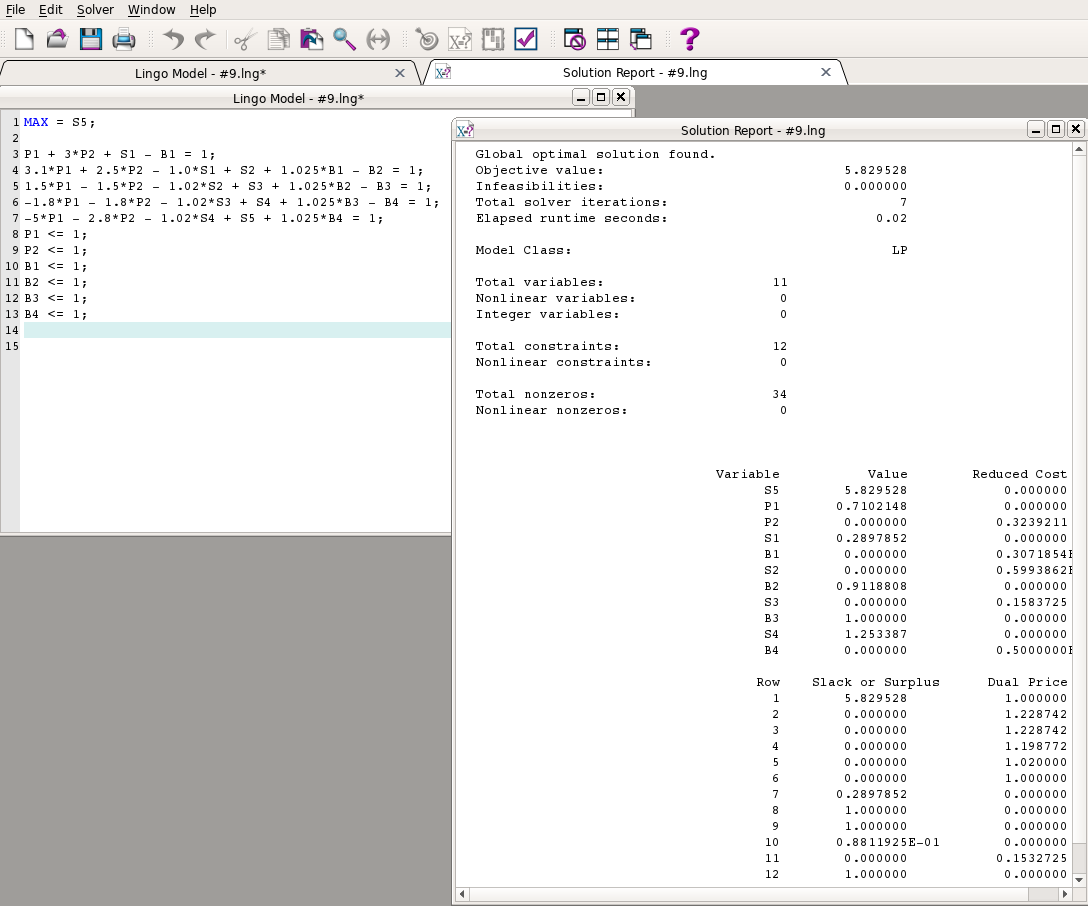
\includegraphics[width=0.7\textwidth]{images/9.png}
\end{figure}


\end{frame}

\begin{frame}[label={sec:org9c62e72}]{}
%%\begin{frame}
\frametitle{Problem 9: Final Solution}

S1 = 0.28\\
S2 = 0\\
S3 = 0\\
S4 = 1.25\\
S5 = 5.82\\
P1 = 0.81\\
P2 = 0\\

B1 = 0\\
B2 = 0.91\\
B3 = 1\\
B4 = 0\\
Z = 5.829528
\end{frame}


\begin{frame}[label={sec:org9c62e72}]{}
%%\begin{frame}
\frametitle{Problem 9: Final Analysis}

The solution shows that BiSi = 0, meaning tha you cannot borrow and also end up with surplus un any quarter. The result makes sense because the cost of borrowing \textcolor{red}{2.5\%} is higher than the return on surplus funds \textcolor{red}{2\%}


\end{frame}


\section{Problem 10}
\label{sec:org92dd686}

\begin{frame}
\frametitle{Problem 10}

In anticipating your child's considerable college spending, a couple has initiated an annual investment program on the day the child turned eight, which will continue until he turns \textcolor{red}{18}. The couple estimates that they can invest the following amounts at the beginning of each year:
\begin{figure}
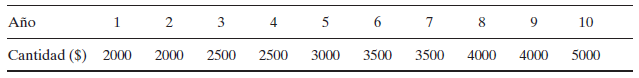
\includegraphics[width=0.7\textwidth]{images/io5.PNG}
\end{figure}

\end{frame}

\begin{frame}[label={sec:org9c62e72}]{}
%%\begin{frame}
\frametitle{Problem 10}
\framesubtitle{cont}

To avoid unpleasant surprise, the couple chooses to invest with security in the following options:

1) Savings insured with annual return of \textcolor{red}{7.5\%} (profit)\\
2) \textcolor{red}{Government bonds for 6 years}, which produce \textcolor{red}{7.9\%} and have a current market price equal to \textcolor{red}{98\%} of the nominal value. (1-5) years.\\
 3) \textcolor{red}{Municipal bonds at 9 years}, which produce \textcolor{red}{8.5\%} with a current market price of \textcolor{red}{1.02} times the nominal value. (1-2) years.
\begin{figure}

\includegraphics[width=0.5\textwidth]{images/J.jpg}
\end{figure}

\end{frame}

% Analysis problem 10

\begin{frame}[label={sec:orge9abdcb}]{}
\frametitle{Problem 10: decision variables }

Ai = savings assured i = 1, 2, 3, 4, 5, 6, 7, 8, 9, 10\\
BGi = Government bonds i = 1, 2, 3, 4, 5\\
BMi = Municipal Bonds i = 1,2

\end{frame}

\begin{frame}[label={sec:orge9abdcb}]{}
%%\begin{frame}

\frametitle{Problem 10: Objective Function }
Maximize\\[1em]

Z =  1.075A10 + 1.079Bg5 + 1.085Bm2


\end{frame}

\begin{frame}[label={sec:orge9abdcb}]{}
\frametitle{Problem 10: Constrains }
\textcolor{red}{Year 1 :} 2000=A1+0.98Bg1+1.02Bm1\\

\textcolor{red}{Year 2 :} 2000+1.075A1=A2+0.98Bg2+1.02Bm2\\

\textcolor{red}{Year 3 :} 2500+1.075A2=A3+0.98Bg3+1.02Bm3\\

\textcolor{red}{Year 4 :} 2500+1.075A3=A4+0.98Bg4+Bm4\\

\textcolor{red}{Year 5 :} 3000+1.075A4=A5+0.98Bg5+Bm5\\

\textcolor{red}{Year 6 :} 3500+1.075A5=A6\\

\textcolor{red}{Year 7 :} 3500 + 1.075A6 + 1.079*0.98Bg1=A7\\

\textcolor{red}{Year 8 :} 4000+1.075A7+1.079*0.98Bg2 = A8\\

\textcolor{red}{Year 9 :} 4000+1.075A8+1.079*0.98Bg3=A9\\

\textcolor{red}{Year 10 :} 5000+1.075A9+1.079*0.98Bg4+1.085Bm1=A10

\end{frame}

\begin{frame}[label={sec:orge9abdcb}]{}
\frametitle{Problem 10: Full Model }
\textcolor{red}{Maximize}\\[1em]
Z =  1.075A10 + 1.079Bg5 + 1.085Bm2\\[1em]
\textcolor{red}{subject to:}\\[1em]
2000=A1+0.98Bg1+1.02Bm1\\

2000+1.075A1=A2+0.98Bg2+1.02Bm2\\

2500+1.075A2=A3+0.98Bg3+1.02Bm3\\

2500+1.075A3=A4+0.98Bg4+Bm4\\

3000+1.075A4=A5+0.98Bg5+Bm5\\

3500+1.075A5=A6\\

3500 + 1.075A6 + 1.079*0.98Bg1=A7\\

4000+1.075A7+1.079*0.98Bg2 = A8\\

4000+1.075A8+1.079*0.98Bg3=A9\\

5000+1.075A9+1.079*0.98Bg4+1.085Bm1=A10
\end{frame}


\begin{frame}[label={sec:orge9abdcb}]{}

\frametitle{Problem 10: Solution with Lingo }
%\textcolor{yellow}{Model problem}\\
\begin{figure}
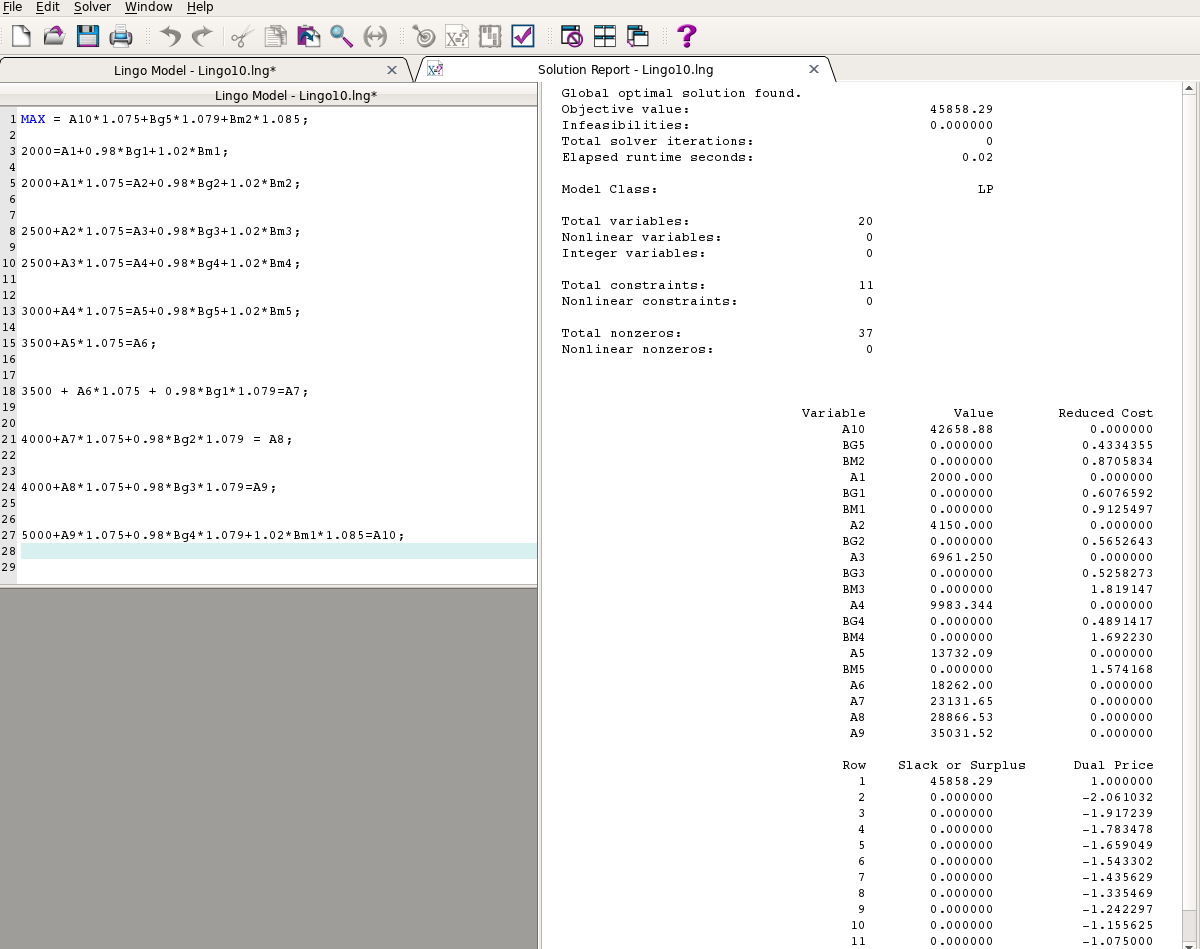
\includegraphics[width=0.7\textwidth]{images/10.png}
\end{figure}


\end{frame}

\begin{frame}[label={sec:org9c62e72}]{}
%%\begin{frame}
\frametitle{Problem 10: Final Solution}

A1 = 2000\\
A2 = 4150\\
A3 = 6961\\
A4 = 9983.34\\
A5 = 13732.09\\
A6 = 18262\\
A7 = 231313.65\\
A8 = 28866\\
A9 = 35031\\
A10 = 42658.88\\

\end{frame}

\begin{frame}[label={sec:org9c62e72}]{}
%%\begin{frame}
\frametitle{Problem 10: Final Solution}
\framesubtitle{cont}

BG1 = 0\\
BG2 = 0\\
BG3 = 0\\
BG4 = 0\\
BG5 = 0\\
BM1 = 0\\
BM2 = 0\\
BM3 = 0\\
BM4 = 0\\
Z = 45858.29

\end{frame}

%------------------------------------------------

\begin{frame}[label={sec:orgf10214b}]{References}
\bibliography{reforg}
\bibliographystyle{smfplain}
Hamdy A. Taha. (2004). Introducción a la programación Lineal. En Investigación de operaciones(11-67). México: PEARSON Education. 
\end{frame}
\end{document}